\chapter{Results}
\section{Covariance Weighted SNR Maps}

Covariance weighted SNR maps for three perpendicular slices chosen to intersect the fetal brain compartment are shown in
figs. \ref{fig:SNR_tra}, \ref{fig:SNR_cor}, and \ref{fig:SNR_sag}. In each cross section, it can be seen that the fetal
array provides greatly increased SNR in the periphery of the phantom, but only narrowly outperforms the standard array
configuration in the deep central region where the fetus is actually located. In this particular dataset, SNR was
improved by approximately $5\%$ inside the fetal brain compartment in each of the three slices. 

\begin{figure}
\makebox[\textwidth][c]{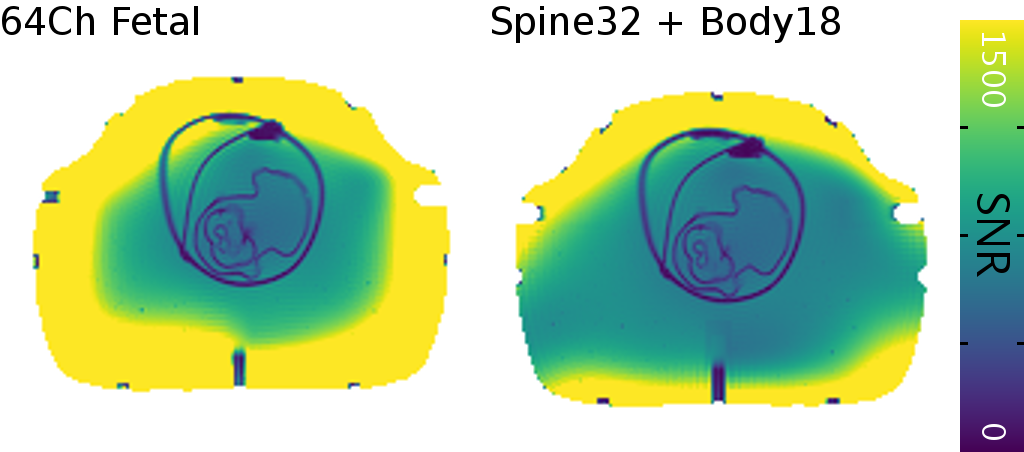
\includegraphics{figures/SNR_TRA_0-1500_viridis.png}}
\caption{Comparative covariance weighted SNR maps, transverse slice through fetal phantom brain.}
\label{fig:SNR_tra}
\end{figure}

\begin{figure}
\makebox[\textwidth][c]{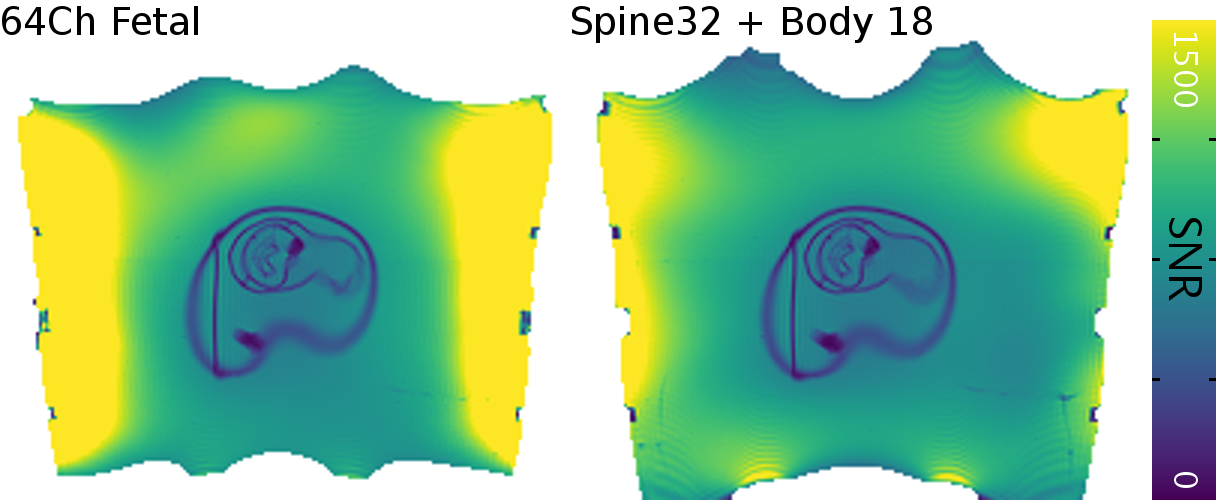
\includegraphics{figures/SNR_COR_0-1500_viridis.png}}
\caption{Comparative covariance weighted SNR maps, coronal slice through fetal phantom brain.}
\label{fig:SNR_cor}
\end{figure}

\begin{figure}
\makebox[\textwidth][c]{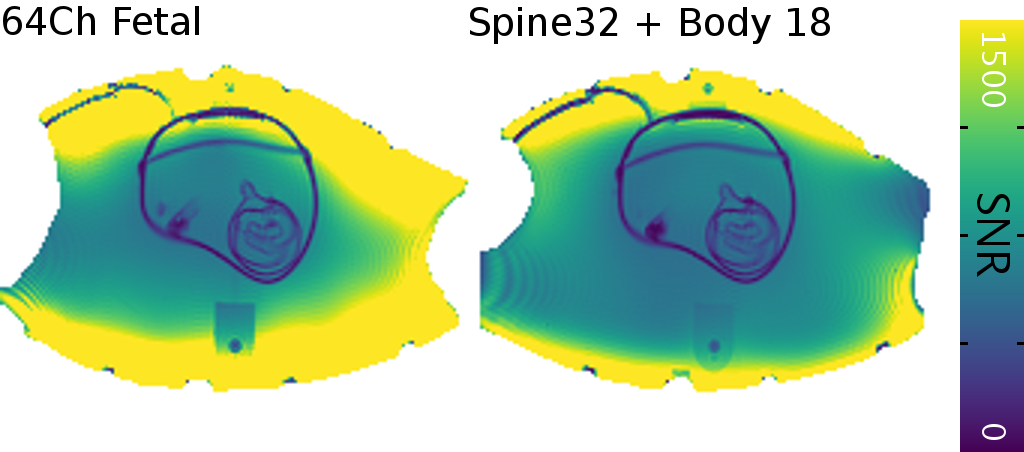
\includegraphics{figures/SNR_SAG_0-1500_viridis.png}}
\caption{Comparative covariance weighted SNR maps, sagital slice through fetal phantom brain.}
\label{fig:SNR_sag}
\end{figure}

\section{Inverse G-Factor Maps}
As compared to the standard combination of the 32 channel spine array and 18 channel flexible body array, the 64 channel
fetal coil allows increase in SENSE acceleration factor from four to five in the right-left direction (figs.
\ref{fig:gfactor_tra_rl}, \ref{fig:gfactor_cor_rl}) and $3$ to $4$ in the head-foot direction (figs.
\ref{fig:gfactor_cor_hf}, \ref{fig:gfactor_sag_hf}) while maintaining acceptably low noise amplification levels. Both
array configurations have poor acceleration capability in the anterior-posterior direction (figs.
\ref{fig:gfactor_tra_ap}, \ref{fig:gfactor_sag_ap}). Note that in order to increase contrast in the relevant range, the
color scale on these maps goes from $0.5$ to $1$, not $0$ to $1$.

Figure \ref{fig:gfactor_cor_hf_rl} shows inverse SENSE g-factor maps for 2D acceleration in the head-foot and left-right
directions, comparing array performance at $R=(3,4)$ and $R=(4,5)$. This comparison was chosen to highlight the best
case improvement in acceleration capability provide by the fetal coil. Inside a large central ROI covering the entire
fetus, the fetal coil maintains $g\le1.5$ with $R=4,5$ while the product array only achieves $g\le3.9$ In the same ROI,
they have mean inverse g-factors ($1/g$) of $0.82$ and $0.43$, respectively. Roughly speaking, the fetal coil has noise
amplification levels at $R=(4,5)$ that are comparable to the standard array configuration at $R=(3,4)$. This represents
a $67\%$ increase in overall acceleration factor.

\begin{figure}
\makebox[\textwidth][c]{\includegraphics{figures/{gfactor_TRA_RL_2-3-4-5-6_0.5-1_viridis}.png}}
\caption{Comparative inverse SENSE g-factor maps, transverse slice through fetal phantom brain, acceleration in
    right-left direction.}
\label{fig:gfactor_tra_rl}
\end{figure}

\begin{figure}
\makebox[\textwidth][c]{\includegraphics{figures/{gfactor_TRA_AP_2-3-4-5-6_0.5-1_viridis}.png}}
\caption{Comparative inverse SENSE g-factor maps, transverse slice through fetal phantom brain, acceleration in
    anterior-posterior direction.}
\label{fig:gfactor_tra_ap}
\end{figure}

\begin{figure}
\makebox[\textwidth][c]{\includegraphics{figures/{gfactor_COR_RL_2-3-4-5-6_0.5-1_viridis}.png}}
\caption{Comparative inverse SENSE g-factor maps, Coronal slice through fetal phantom brain, acceleration in right-left direction.}
\label{fig:gfactor_cor_rl}
\end{figure}

\begin{figure}
\makebox[\textwidth][c]{\includegraphics{figures/{gfactor_COR_HF_2-3-4-5-6_0.5-1_viridis}.png}}
\caption{Comparative inverse SENSE g-factor maps, coronal slice through fetal phantom brain, acceleration in head-feet direction.}
\label{fig:gfactor_cor_hf}
\end{figure}

\begin{figure}
\makebox[\textwidth][c]{\includegraphics{figures/{gfactor_SAG_HF_2-3-4-5-6_0.5-1_viridis}.png}}
\caption{Comparative inverse SENSE g-factor maps, sagital slice through fetal phantom brain, acceleration in head-feet direction.}
\label{fig:gfactor_sag_hf}
\end{figure}

\begin{figure}
\makebox[\textwidth][c]{\includegraphics{figures/{gfactor_SAG_AP_2-3-4-5-6_0.5-1_viridis}.png}}
\caption{Comparative inverse SENSE g-factor maps, sagital slice through fetal phantom brain, acceleration in
    anterior-posterior direction.}
\label{fig:gfactor_sag_ap}
\end{figure}

\begin{figure}
    \makebox[\textwidth][c]{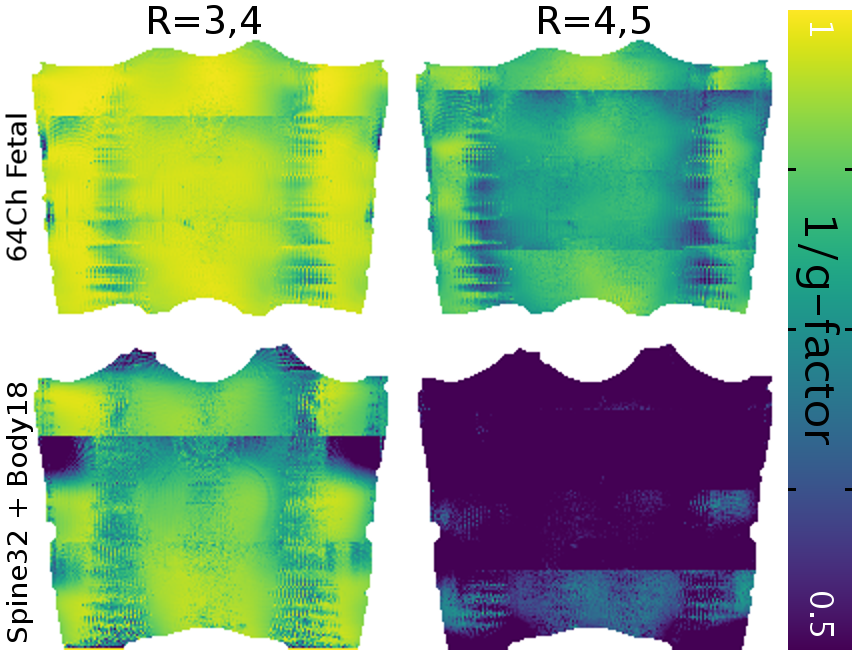
\includegraphics{{figures/gfactor_COR_HF_RL_3-4_4-5_0.5-1_viridis}.png}}
\caption{Comparative inverse SENSE g-factor maps, coronal slice through fetal phantom brain, acceleration in head-feet,
    right-left directions.}
\label{fig:gfactor_cor_hf_rl}
\end{figure}

\section{Noise Matrices}
Figure \ref{fig:noise_cov} shows the absolute value of a noise covariance matrix $\Psi$ calculated from this dataset.
Figure \ref{fig:noise_cor} shows the same data normalized along the diagonal so that the element with indices $j,k$ is
the correlation coefficient for channels $i$ and $k$. The correlation coefficient is equal to 1 when $j=k$.

The average off diagonal correlation coefficient is $0.051$, and the maximum is $0.38$.

Looking at the correlation coefficient matrix, several clearly defined regions of moderate correlation are apparent,
with almost no correlation between different regions. The groupings follow the separation of elements into different
array panels. From top left to bottom right, we see channels from the right side wing, left side wing,
abdomen panel, and back panel.

\begin{figure}
    \makebox[\textwidth][c]{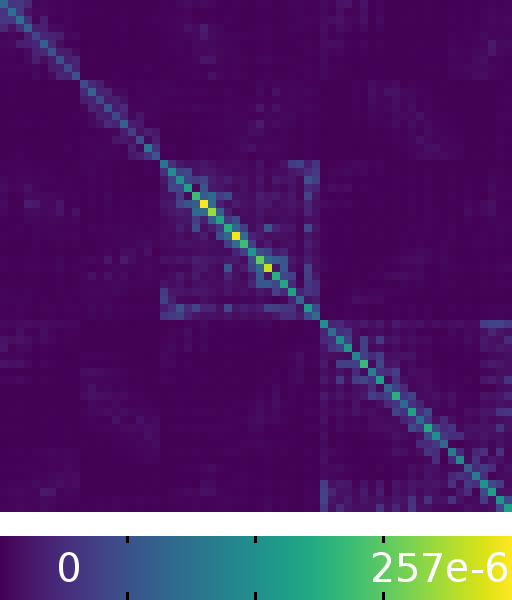
\includegraphics[width=4in]{figures/noise_cov.png}}
    \caption{Absolute value of noise covariance matrix ($|\Psi|$).}
\label{fig:noise_cov}
\end{figure}

\begin{figure}
    \makebox[\textwidth][c]{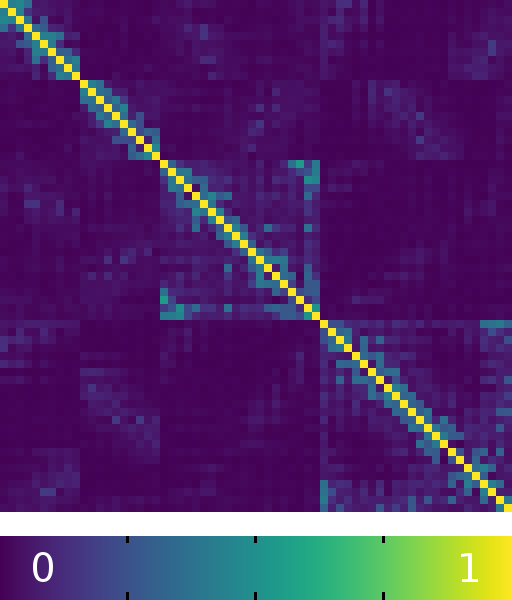
\includegraphics[width=4in]{figures/noise_cor.png}}
    \caption{Absolute value of inter-channel noise correlation coefficients ($|\sqrt{diag(\Psi)}^{-1} \cdot \Psi \cdot
    \sqrt{diag(\Psi)}|$).}
\label{fig:noise_cor}
\end{figure}

\section{Per-Element SNR}
Figure \ref{fig:loop_snr_contributions} is a 1:4 scale diagram of the actual loop geometry used in the fetal array.
Displayed inside each loop is the mean SNR of that channel inside the fetal brain ROI. It can be seen that elements in
the back panel contributed mos to overall SNR in the fetal brain compartment, followed by the belly panel and side wings.

\begin{figure}
\makebox[\textwidth][c]{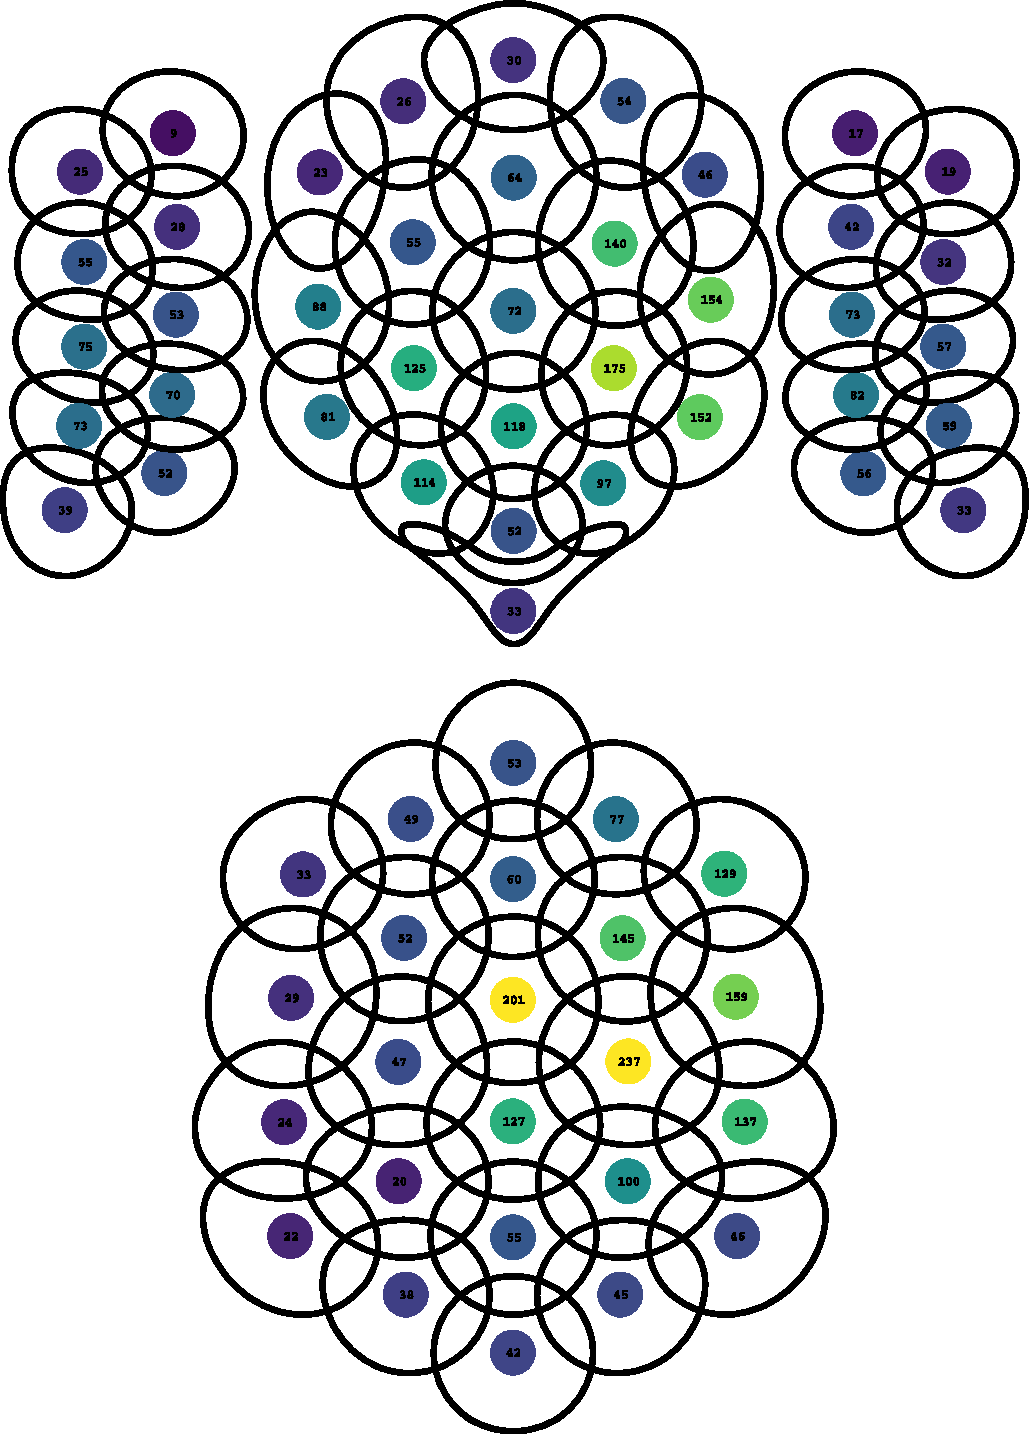
\includegraphics{figures/loop_snr_contributions.pdf}}
\caption{Mean Single Element SNR values Inside the Fetal Phantom Brain (Top:Abdomen Panel and Side Wings, Bottom: Back
panel)}
\label{fig:loop_snr_contributions}
\end{figure}
